%%% Fiktivní kapitola s ukázkami sazby

\chapter{Návrh}

Kapitola návrh se věnuje dvou tématům. V první části se věnuje návrhu uživatelského rozhraní a přechodů mezi obrazovkami. V druhé části se věnuje tradičnějšímu chápání slova návrh ve vývoji, a to softwarové architektuře. Cílem návrhu je vytvořit postup, jakým se má při implementaci postupovat.

\section{Uživatelské rozhraní}

Návrh uživatelského rozhraní je disciplínou softwarového inženýrství, která se věnuje návrhu uživatelského rozhraní na koncepční úrovni. Při vytváření uživatelského rozhraní je nutno brát v potaz požadavky uživatelů, aby nebylo ubíráno na efektivitě aktivity uživatele v aplikaci. Cílem je navrhnout uživatelské rozhraní pro uživatele rychlo uchopitelné a přehledné. V disciplíně návrhu uživatelského rozhraní se využívá mnoho modelovacích technik, např. prototypování a drátěné modely. Pro správné posouzení efektivnosti uživatelského rozhraní je nutno tyto modely konfrontovat s potenciálními uživateli a sledovat jejich reakce a přpomínky a reflektovat je v následujících iteracích návrhu uživatelského rozhraní. 

Pro tuto práci byla zvolena technika drátěných modelů (tzv. wireframe), schematickým nákresem prvků na obrazovce a jakým způsobem do sebe zapadají \cite{garrett2010elements}. Tyto návrhy jsou ušetřeny komentářů, které součástí wireframů někdy bývají. V rámci této práce nebylo možno provádět studie mezi potenciálními uživateli, byl zvolen alternativní způsob inspirace známými UI elementy, které jsou přítomny v jiných aplikacích. 


% https://www.academia.edu/6511543/The_Elements_of_User_Experience_User-Centered_Design_for_the_Web_and_Beyond_Second_Edition p. 128

\subsection{Onboarding, přihlášení, registrace}

\begin{figure}[H]
	\begin{center}
		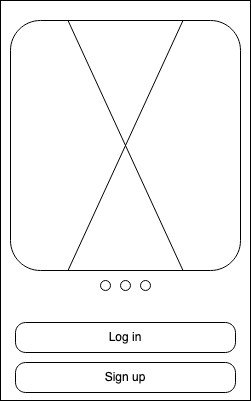
\includegraphics[width=70mm]{img/wf_onboarding.png}
		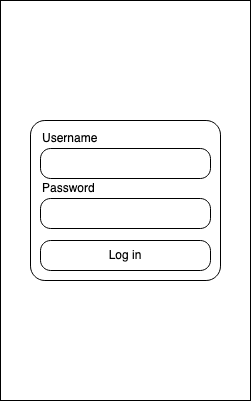
\includegraphics[width=70mm]{img/wf_login.png}
	\end{center}
	\caption[Wireframe přihlášení a onboarding obrazovky]{Wireframe onboarding a přihlašovací obrazovky -- zdroj: autor}
\end{figure}

Pro přihlašovací obrazovku byl zvolen koncept tzv. onboardingu, praktiky popisující funkce aplikace a výhody založení účtu. Onboarding lze také chápat jako náhradu aplikačního návodu. Onboarding může být prováděn mnoha způsoby, jako nejsnadněji řešitelný byl vybrán tzv. carousel, seznam posouvatelných panelů, kde každý z nich obsahuje určité informace o mobilní aplikaci. Pro přihlašovací obrazku byl zvolen očekávatelný klasický formát přihlašovacího dialogu. Pro registraci byl využit tzv. web view, komponenta, co zobrazí webový prohlížeč svázaný s aplikací. Registrace se tedy provádí přes stávající webovou aplikaci. Důvodem tohoto rozhodnutí je absence API pro vytváření uživatelských účtu, ale zároveň i předpoklad, že uživatel mobilní aplikace bude i zároveň uživatelem aplikace webové.

\subsection{Mapová koncepce}

Hlavní obrazovkou aplikace byla zvolena obrazovka s mapou, aby odpovídala očekávání uživatelů webové aplikace Anitra, kde hlavní obrazovkou je taktéž mapa. Veškeré kontrolky, které by se daly zobrazit jako separátní stránky, se zobrazují v modálních oknech nad obrazovkou, což je opět koncepce vycházející z již hotové webové aplikace. Aplikace tedy rovnou splní jeden ze zmíněných případů užití při zapnutí, a to kontrolu posledních pozic trackerů a případné odfiltrování pro uživatele nezajímavých trackerů způsoben srovnatelným s aktuálním řešením, čímž by se dalo očekávat zkrácení doby učení uživatelů aplikace. Na mapě se zobrazují individuální poslední pozice trackerů uživatele, aktuálnost poslední pozice je odstupňována dle času a barvy ikony, konzistentně s aktuálním řešením. V poslední pozici se zobrazí základní informace o trackeru -- název, lokalita poslední pozice. Po klepnutí na poslední pozici se zobrazí detail objektu, ze kterého uživatel může spouštět další akce.


\begin{figure}[H]
	\begin{center}
		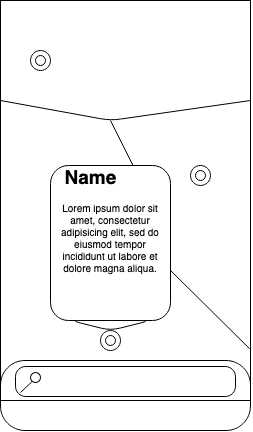
\includegraphics[width=70mm]{img/wf_lastpos.png}
		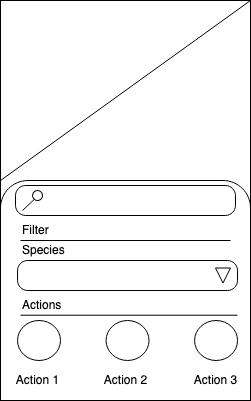
\includegraphics[width=70mm]{img/wf_filter.png}
	\end{center}
	\caption[Wireframe poslední pozice a filtrování mapy]{Wireframe poslední pozice a filtrování mapy -- zdroj: autor}
\end{figure}

Pro navigaci v aplikaci je potřeba zavést základní menu, které uživateli umožní nejpodstatnější akce docílit v rozmezí pár uživatelských interakcí. Do aplikace bylo přidáno menu ve formě vyjížděcí kontrolky (realizované knihovnou rn-sliding-up-panel) s full-text vyhledávačem v hlavičce. Po zadání textu do vyhledávače se prozkoumají názvy všech trackerů a na mapě (či v dalších přehledových kontrolkách) zůstanou pouze relevantní trackery. Po vysunutí menu nahoru se zobrazí další možnost filtrování, a to klíčový výběr podle druhu. Filtry fungují v kombinaci ve formě logické spojky A. Pod filtrem druhu se nachází seznam akcí, které uživatel může provést. 

\subsection{Detail trackeru}

\begin{figure}[H]
	\begin{center}
		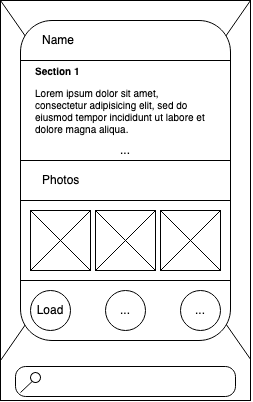
\includegraphics[width=70mm]{img/wf_trackingdetail.png}
	\end{center}
	\caption[Wireframe detailu trackeru]{Wireframe detailu trackeru -- zdroj: autor}
\end{figure}

Po vybrání trackeru v mapě nebo v seznamu trackerů (viz dále) se uživateli zobrazí modální okno s popisem, základními informacemi, fotogalerií a seznamem akcí, které uživatel může s trackerem provést, v prvotní verzi aplikace pouze načíst trasu za posledních 30 dní (nebo do limitu 100 pozic). Ze stejného okna lze načtenou trasu skrýt.

\subsection{Kontextové menu a podobrazovky}

\begin{figure}[H]
	\begin{center}
		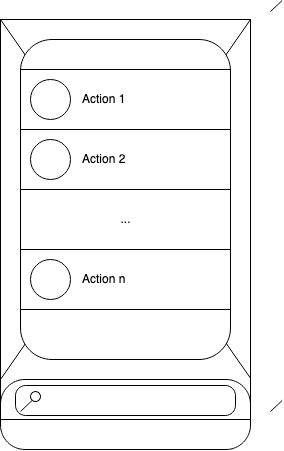
\includegraphics[width=70mm]{img/wf_contextmenu.png}
	\end{center}
	\caption[Wireframe kontextového menu]{Wireframe kontextového menu -- zdroj: autor}
\end{figure}

Kvůli způsobu provedení aplikace nebylo mnoho míst, kam přehledně uložit ovládací prvky. Některé ovládací prvky jsou také provázány s kliknutím do mapy. Z tohoto důvodu byl zvolen koncept kontextového menu nad mapou. Po dlouhém klepnutí na hlavní mapu se zobrazí seznam veškerých dostupných akcí. V seznamu jsou i globální (tedy nekontextové) akce, např. odhlášení, zobrazení seznamu trackerů, výběr mapových podkladů, stáhnutí off-line map. Kontextové menu se zobrazí v klasickém modálním okně a dá se odvolat kliknutím mimo okno nebo na jakýkoliv ovládací prvek vně.

\begin{figure}[H]
	\begin{center}
		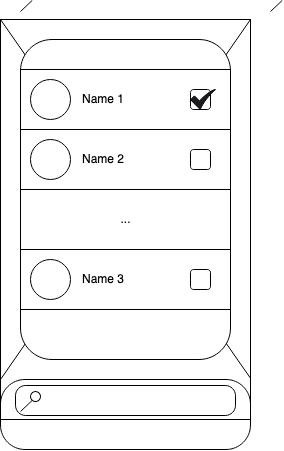
\includegraphics[width=70mm]{img/wf_list.png}
	\end{center}
	\caption[Wireframe seznamu trackerů]{Wireframe seznamu trackerů -- zdroj: autor}
\end{figure}

Pro seznam trackerů byla zvolena seznamová komponenta s hlavičkami oddělující jednotlivé druhy, kvůli konzistenci s webovou aplikací. Kliknutím na položk u v seznamu se zobrazí detail trackeru a kliknutím na zaškrtávací tlačítko se načte trasa zařízení.

Stáhnutí off-line regionu map se aktivuje po kliknutí na položku v kontextovém menu, pokud je uživatel dostatečně přiblížen v mapě. Pro uživatele nemá smysl stahovat regiony výrazně větší než 1 km$^2$, což lze omezit právě např. minimálním tzv. \emph{zoom levelem} mapy. Běžné rasterové (tedy především satelitní) mapy jsou klientksým softwarům indexovány v trojrozměrné struktuře ve formátu \emph{z-x-y}, kde z udává zoom level a x a y 2D souřadnice daného mapového čtverce. Tato struktura v podstatě odpovídá datové strutkuře \emph{quadtree}, roste tedy exponenciálně počet čtverečků ve kterých se vyskytuje vybraná plocha, zatímco velikost jednotlivých čtverečků v bytech je v podstatě srovnatelná. Pro ušetření místa na klientovi byl vybrán tedy přístup s omezením vybrané plochy nastavením minimálního zoom levelu. Uživatel tak může prakticky stahovat maximálně několik stovek mapových čtverečků, čímž by nemělo dojít k nedostatku místa na straně uživatele. Před stáhnutím bude uživateli zobrazen dialog, ve kterém se uživateli zobrazí počet čtverečků ke stáhnutí a odhadovaná velikost v bytech. Po potvrzení ze strany uživatele se zobrazí indikátor zobrazující počet státhnutých čtverečků k celkovému počtu. Při zadávání se také uživateli zobrazí na mapě již stáhnuté regiony označené červeným čtvercem.

\section{Aplikační architektura}

%Clements, Paul; Felix Bachmann; Len Bass; David Garlan; James Ivers; Reed Little; Paulo Merson; Robert Nord; Judith Stafford (2010). Documenting Software Architectures: Views and Beyond, Second Edition. Boston: Addison-Wesley. ISBN 978-0-321-55268-6.

Aplikační (resp. softwarová) architektura popisuje strukturu softwarového systému. Struktura softwarového systému obsahuje softwarové elementy, jejich vztahy a vlastnosti elementů a jejich vlastností \cite{clements2010documenting}. Přístupy k této disciplíně se liší dle metodiky vývoje softwaru, rigozórní metody preferují architekturu dopředu pevně formulovat, zatímco více agilní metodiky pravý opak. V rámci této práce softwarová architektura nebyla řešena příliš do podrobna, jelikož se jedná o velmi malou aplikaci a úmyslem bylo dodat produkt co nejdříve. Cílem bylo navrhnout koncept bez zbytečných duplikacích kódu, možností centralizovaného čtení a zápisu do cache, volání API z jednoho místa a přehlednost kódu.

\subsection{Základní koncepce}

Pro řešení aplikace byly zvoleny architektonické vzory, tedy typické architektury, které se v návrhu softwarových architektur vyskytují. Aplikace byla navrhnutá jako dvouvrstvá klient-server aplikace, kde první vrstva zajišťuje operaci s daty (modelová vrstva, podkapitola Datové zdroje a entity) a druhá vrstva správné zobrazení (prezentační vrstva, podkapitola Komponenty). Tento koncept byl zvolen díky plnému splnění architektonických nároků malé aplikace a komponentové architektuře React, přičemž bylo zajištěno, že je dodržen princip toku dat (z modelů do komponent) a událostí (z komponent do modelů). 

\subsection{Datové zdroje a entity}

Aplikace je ze své podstaty klientem webové služby poskytované platformou Anitra, data z trackerů jiným způsobem optimálně získat nelze. Komunikace se vzdáleným serverem probíhá pomocí Hyper Text Transfer Protocolu, za pomocí tzv. REST API formátu, přičemž zprávy ze strany serveru jsou serializovány do formátu JSON, které v aplikaci odpovídají entitám (vyměněné zprávy jsou většinou počtem atributů nadmnožinou, mobilní aplikace nepotřebuje všechna data). Pro každou doménovou oblast bylo v aplikaci vytvořeno tzv. uložiště -- třída, která plní určité business požadavky, přičemž prezentační vrstva nepotřebuje vědět, jakým způsobem byla data získána či předaná data zpracována. Název uložiště byl zvolen právě z důvodu, že třídy zajišťují i cachování objektů.

\begin{figure}[H]
	\begin{center}
		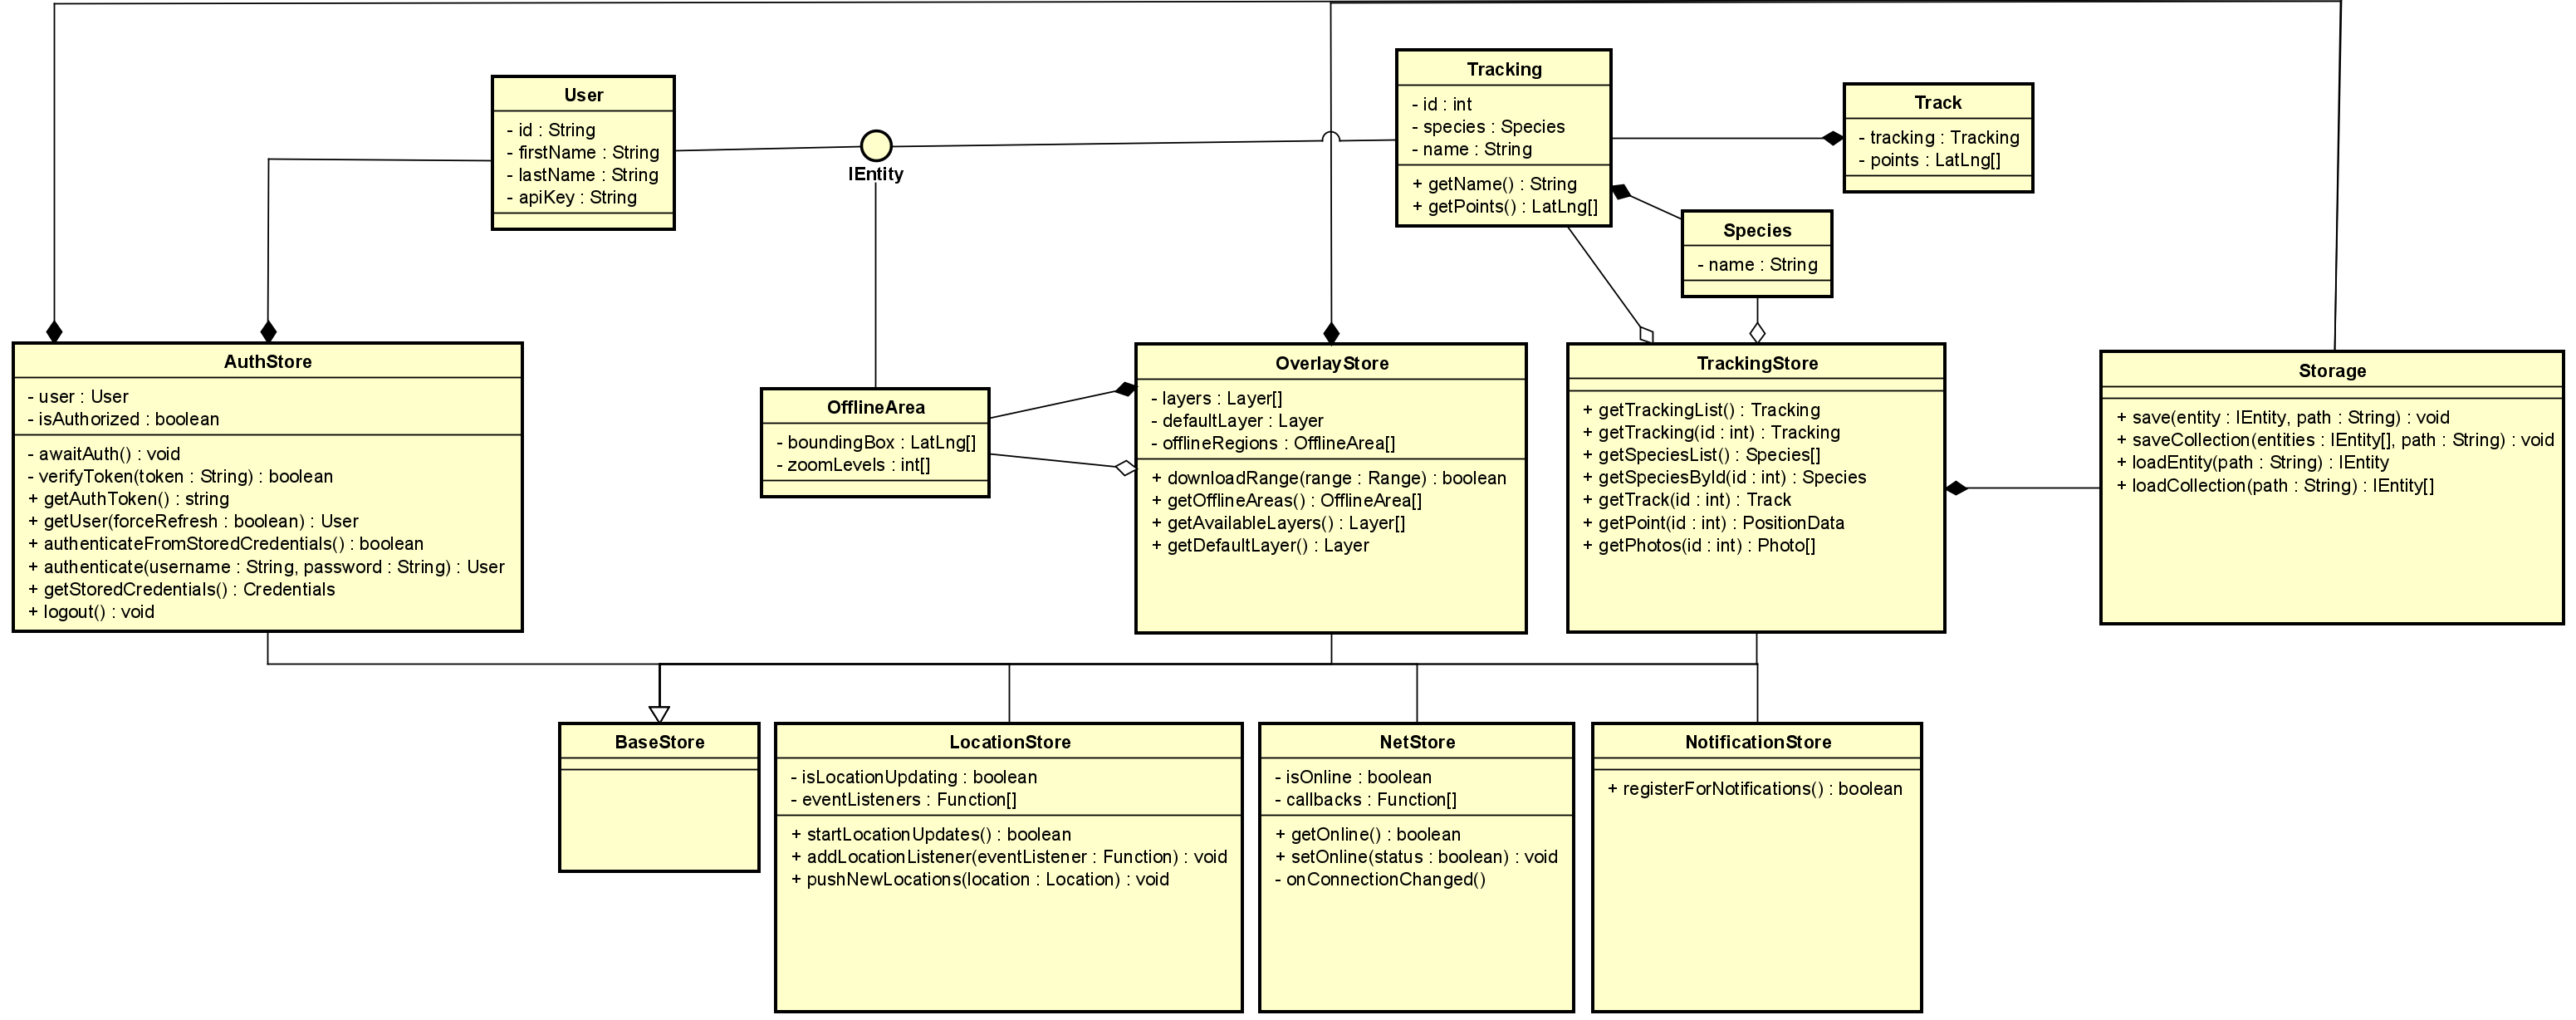
\includegraphics[width=145mm]{img/classdiagram.png}
	\end{center}
	\caption[Class diagram datových zdrojů a entit]{Class diagram -- zdroj: autor}
\end{figure}

Pro aplikaci byly navrhnuty následující datové zdroje:

\begin{itemize}
	\item BaseStore -- základní třída pro společnou funkcionalitu,
	\item AuthStore -- třída poskytující metody pro autentifikaci uživatele,
	\item LocationStore -- třída zpracovávající získávání a ukládání GPS pozic,
	\item NetStore -- třída zpracovávající události spojené s připojením a odpojením k internetu,
	\item NotificationStore -- třída zpracovávající registraci k notifikacím,
	\item OverlayStore -- třída zajišťující mapové podklady,
	\item TrackingStore -- třída zajišťující akce spojené s jednotlivými trackery.
\end{itemize}

Na datové zdroje navazují entity, objekty, se kterými komponenty i datové zdroje pracují. Nejpodstatnější datové zdroje jsou uvedeny níže:

\begin{itemize}
	\item Tracking -- informace o trackeru,
	\item Species -- kontejner pro názvy druhu,
	\item Track -- informace o trase zařízení,
	\item User -- uživatel aplikace,
	\item OfflineRegion -- informace o stáhnutých mapových podkladech.
\end{itemize}

\subsubsection{Cache}


Uložiště pro každý požadavek provádí následující sekvenci rozhodnutí: pokusí se načíst výsledek (entitu) z cache a prověřit, že není starší než daný časový limit, aby byla dodržena aktuálnost dat. V případě že je stáří entity přes časový limit a uživatel je připojený k internetu, uživateli se vrátí čerstvá odpověď z API. V případě že uživatel připojený k síti není, vrátí se uložená odpověď, případně chyba, pokud žádná není. Chyba je odchycena v uživatelském rozhraní a uživateli se zobrazí hláška, že tento zdroj nebyl uložen do aplikační cache. V případě že soubor v cache není a uživatel je připojen k internetu, z API se entita získá a uloží na disk. Tímto se zajistí dostupnost aktuálních dat v případě že uživatel připojený k internetu je a dostupnost dat v případě že není. V obrázku \ref{cachediagram} je celý proces vyznačen vývojovým diagramem.

\begin{figure}[H]
	\begin{center}
		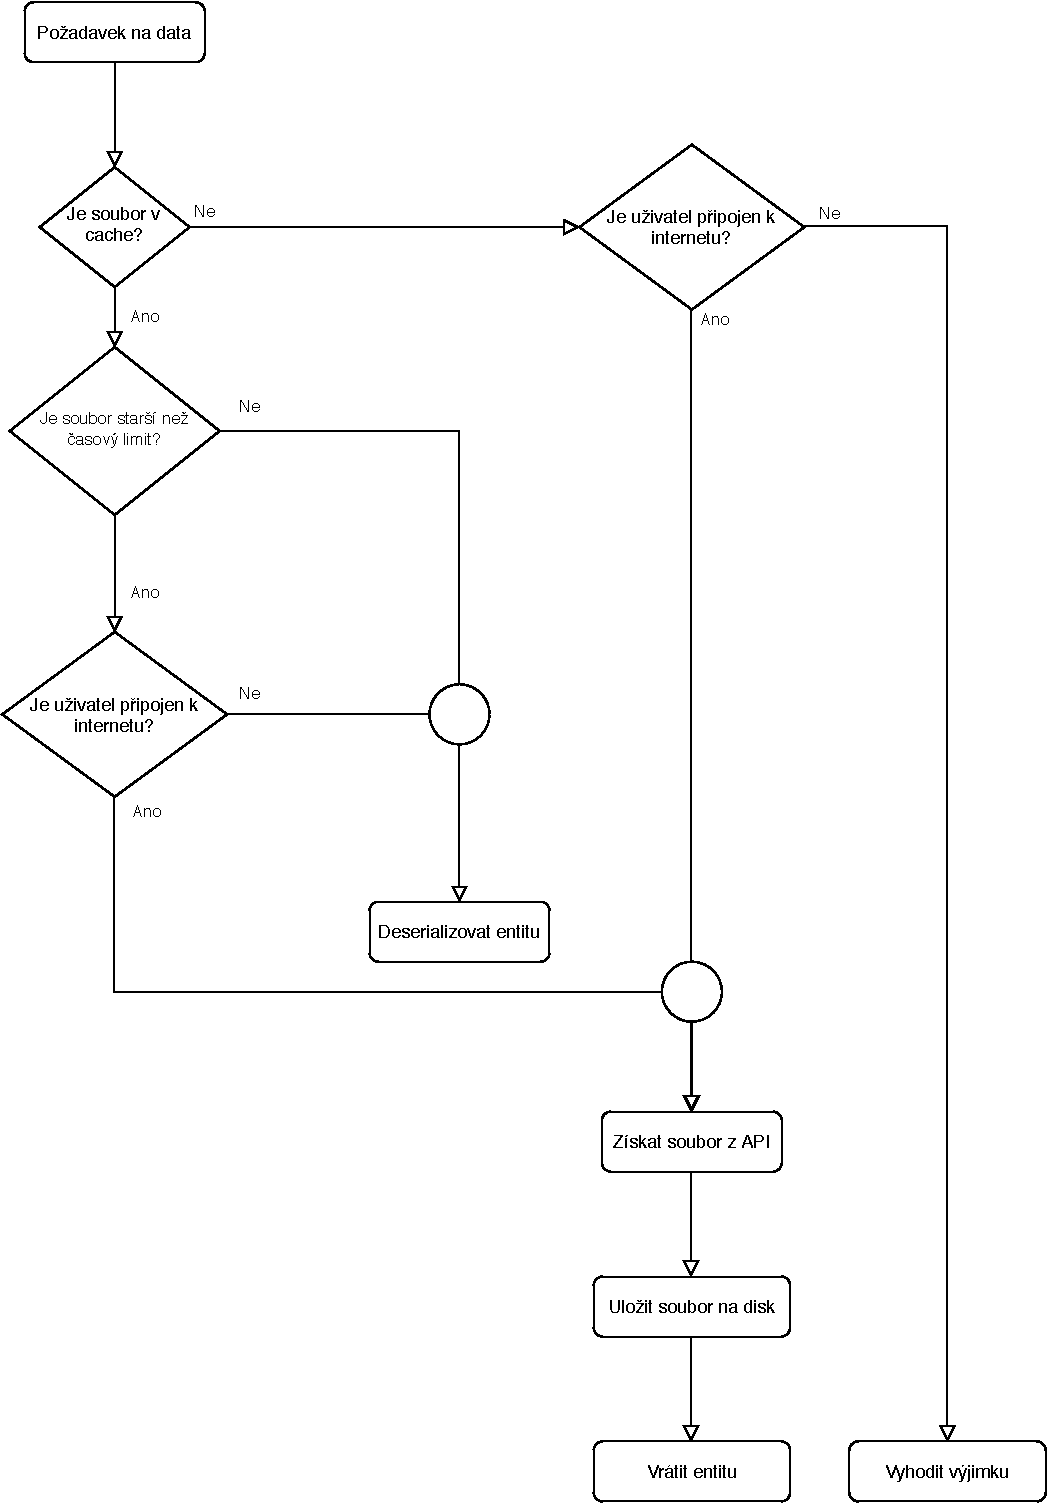
\includegraphics[width=145mm]{img/cache.pdf}
	\end{center}
	\caption[Cache -- vývojový diagram]{Vývojový diagram cache -- zdroj: autor}
	\label{cachediagram}
\end{figure}


\subsection{Komponenty}

V předchozích kapitolách byl zmíněn základ komponentového systému React, který aplikace využívá. Komponenty jsou samostatné (a často znovupoužitelné) části aplikace s datovými vstupy a reagující na události, ať už uživatelského rozhraní či dceřiných komponent. Komponenty v aplikaci lze rozdělit do dvou typů dle funkcí, které plní. První skupinou jsou obrazovky sdružují komponenty neobrazovkového typu (dále subkomponenty) do funkčního celku a předávají jim data a reagují na jejich události. Subkomponenty zpravidla slouží k zobrazování určitých dat nebo uživatelské interakci. Subkomponentám jsou předávána data a s obrazovkami komunikují přes události, je zde tedy zajištěná obousměrná komunikace mezi obrazovkou a komponentou. Předáním dat se zpravidla subkomponenta překreslí bez nutnosti překreslit nesouvisející (sub)komponenty, čímž je splněna tzv. reaktivita aplikace (zajištěna předem zmíněnou knihovnou MobX).

Komponenty jsou strukturovány do složek dle svého typu. Obrazovky jsou uloženy ve složce \emph{src/screens}, subkomponenty se nachází ve složce \emph{src/components}.

\begin{figure}[H]
	\begin{center}
		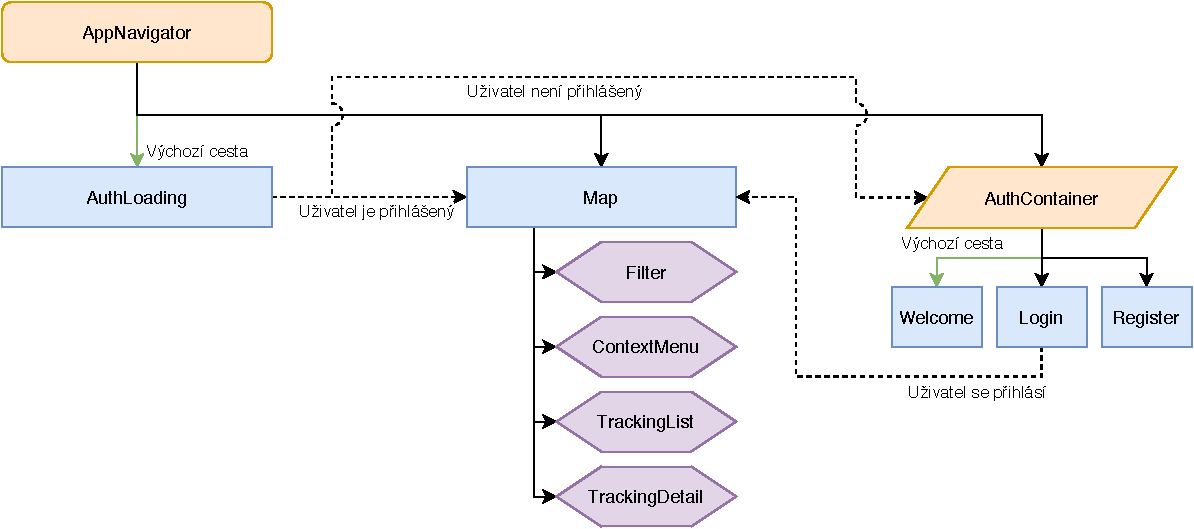
\includegraphics[width=145mm]{img/components.pdf}
	\end{center}
	\caption[Strom komponent]{Strom komponent -- zdroj: autor, klíč níže}
	\label{componenttree}
\end{figure}

\subsubsection{Obrazovky}

Obrazovky v aplikaci se skládají do tzv. navigátorů. Navigátor je komponentou knihovny \emph{react-navigation}, která umožňuje přepínat mezi obrazovkami v reakci na uživatelské interakce nebo události v kódu (ref). Princip práce s navigátory je daný historií knihovny React  a v nomenklatuře i chování odpovídá principům webových stránek. Každá obrazovka je přirovnatelná k webové stránce, navigátor mezi nimi umí přesměrovat a fungují zde koncepty navigačních tlačítek zpět i vpřed. Navigátory se rozlišují dle typů uživatelských interakcí pro přenavigování, v aplikaci se používají pouze dva z mnoha typů. Navigátory lze skládat do sebe a lze se navigovat napříč obrazovkami jiných navigátorů.

Prvním použitým typem je \emph{SwitchNavigator}, který nemá prostředky pro navigaci mezi obrazovkami na základě uživatelských interakcí (např. tlačítko zpět, gesto přetáhnutí po obrazovce), ale pouze z kódu. Tento navigátor je vhodný pro úvodní stránku s rozhodnutí, zda má uživatel být přesměrován na přihlášení nebo do aplikace. V obrázku \ref{componenttree} je uveden v zaobleném obdélníku nahoře pod názvem AppNavigator.

Druhým využitým navigátorem je \emph{StackNavigator}, který funguje na principu zásobníku (ref). Každá nová otevřená obrazovka se přiřadí na vrchol zásobníku a uživatel se může z této obrazovky vždy vrátit na předchozí. Tento navigátor se hodí např. na registraci a přihlášení. Na obrázku \ref{componenttree} je uveden v kosodélníku vpravo pod názvem AuthContainer.

Aplikace bude celá obalena v jednom SwitchNavigatoru, pro jednodušší správu autentizované a neautentizované části aplikace. Výchozí obrazovkou aplikace je \emph{AuthLoading}, která rozhodne, zda se uživatel má přesměrovat do neautentizované části či do autentizované. Neautentizovaná část (pod navigátorem \emph{AuthContainer}) se dále dělí na stránky onboarding (Welcome), přihlášení (Login) a registrace (Register). Mezi neautentizovanými stránkami lze přepínat gestem či tlačítkem zpět. Autentizovaná část (Map) je postavena na mapové koncepci aplikace a není využitý žádný navigátor, ale modální okna tvořená subkomponentami.

\subsection{Subkomponenty}

Subkomponenty vycházejí z předešlých částí návrhu (konkrétněji wireframe) a pro každou komponentu z wireframe bude vytvořena vlastní React komponenta. Pro často používané opakující se fragmenty v GUI lze také využít vlastní komponenty, o tomto bude rozhodnuto v implementaci. Subkomponenty nebyly předem plánovány do stejné úrovně jako obrazovky a mimo subkomponenty definovaé z wireframů byly vytvářeny ad hoc. Některé subkomponenty jsou vyznačeny v obrázku \ref{componenttree} v fialových šestiúhelnících pod obrazovkou Map.
